Computer Management biedt je de mogelijkheid om gebruikers aan te maken. In Computer Management vind je onder \textquote{System Tools} het kopje \textquote{Local Users and Group}. We zien bij \textbf{Users} gelijk een overzicht van alle aanwezige gebruikers op ons systeem. Er zijn standaard al enkele accounts aanwezig. De zogenaamde Built-in accounts en wat administratieve accounts. Bij \textquote{Description} vind je uitleg over het account, waar het voor dient.

Als we in deze omgevind aan account aanmaken, door bij \textbf{Action} voor \textbf{New User...} te kiezen of door op de rechtermuisknop te klikken onder de bestaande gebruikers en dan voor \textbf{New User...} te kiezen, dan kunnen we veel extra data aan een account meegeven.

\begin{minipage}[t]{\linewidth}
\raggedright
\adjustbox{valign=t}{%
	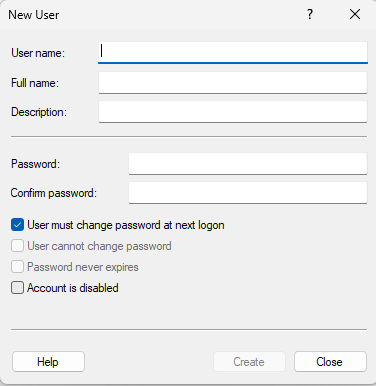
\includegraphics[width=0.99\linewidth]{computer_management-new_user.png}%
}
\end{minipage}

We kunnen een account aanmaken door een gebruikersnaam (Username) op te geven en het account te voorzien van een \textquote{veilig} wachtwoord. Als extra informatie kunnen we bij het aanmaken van het account de volledige naam van de gebruiker meegeven en een beschrijving (Description), zodat we later nog weten waarom dit account aangemaakt is.

Tot slot zijn er een aantal opties bij het aanmaken van een account:
\begin{description}
\item{User must change password at net logon} Dit geeft je de mogelijkheid om voor een nieuw account een simpel wachtwoord te zetten en te zorgen dat de gebruiker zelf zijn eigen wachtwoord kiest.
\item{User can not change password} Kan je gebruiken om zelf een sterk wachtwoord voor de gebruiker te zetten en te zorgen dat de gebruiker het wachtwoord niet kan wijzigen.
\item{Password never expires} Zorgt ervoor dat een wachtwoord nooit verloopt en dus eeuwig geldig blijft (tot jij als beheerder anders beslist of het account verwijderd)
\item{Account is disabled} Is een simpele methode om een account te disablen. Het bestaat dan nog wel, maar kan niet meer gebuikt worden.
\end{description}

